% Created by tikzDevice version 0.12.6 on 2026-08-08 13:32:30
% !TEX encoding = UTF-8 Unicode
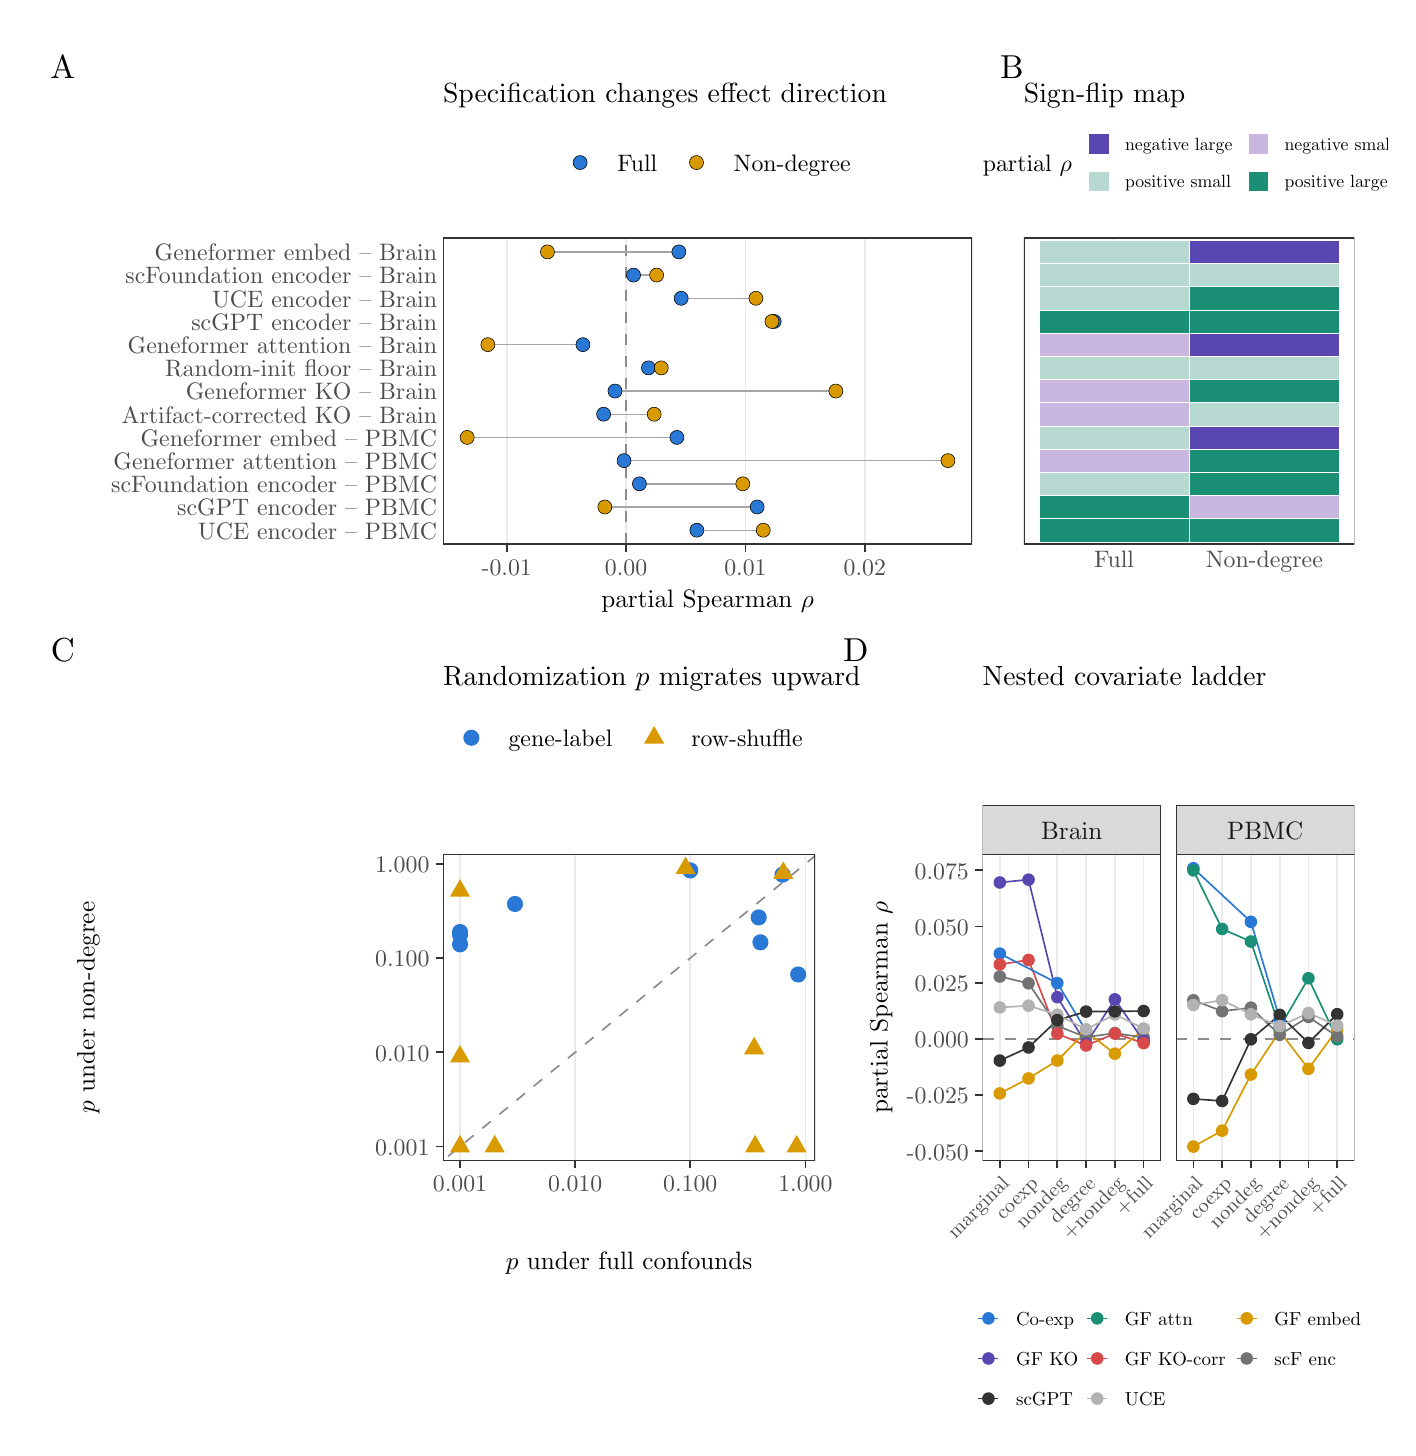
\begin{tikzpicture}[x=1pt,y=1pt]
\definecolor{fillColor}{RGB}{255,255,255}
\path[use as bounding box,fill=fillColor,fill opacity=0.00] (0,0) rectangle (491.44,505.89);
\begin{scope}
\path[clip] (  0.00,  0.00) rectangle (491.44,505.89);
\definecolor{drawColor}{RGB}{255,255,255}
\definecolor{fillColor}{RGB}{255,255,255}

\path[draw=drawColor,line width= 0.6pt,line join=round,line cap=round,fill=fillColor] ( -0.00, -0.00) rectangle (491.44,505.89);
\end{scope}
\begin{scope}
\path[clip] (  4.00,291.25) rectangle (347.23,501.89);
\definecolor{drawColor}{RGB}{255,255,255}
\definecolor{fillColor}{RGB}{255,255,255}

\path[draw=drawColor,line width= 0.6pt,line join=round,line cap=round,fill=fillColor] (  4.00,291.25) rectangle (347.23,501.89);
\end{scope}
\begin{scope}
\path[clip] (347.23,291.25) rectangle (485.44,501.89);
\definecolor{drawColor}{RGB}{255,255,255}
\definecolor{fillColor}{RGB}{255,255,255}

\path[draw=drawColor,line width= 0.6pt,line join=round,line cap=round,fill=fillColor] (347.23,291.25) rectangle (485.44,501.89);
\end{scope}
\begin{scope}
\path[clip] (150.12,319.27) rectangle (341.23,429.89);
\definecolor{fillColor}{RGB}{255,255,255}

\path[fill=fillColor] (150.12,319.27) rectangle (341.23,429.89);
\definecolor{drawColor}{gray}{0.92}

\path[draw=drawColor,line width= 0.6pt,line join=round] (173.12,319.27) --
	(173.12,429.89);

\path[draw=drawColor,line width= 0.6pt,line join=round] (216.25,319.27) --
	(216.25,429.89);

\path[draw=drawColor,line width= 0.6pt,line join=round] (259.38,319.27) --
	(259.38,429.89);

\path[draw=drawColor,line width= 0.6pt,line join=round] (302.51,319.27) --
	(302.51,429.89);
\definecolor{drawColor}{gray}{0.55}

\path[draw=drawColor,line width= 0.6pt,dash pattern=on 4pt off 4pt ,line join=round] (216.25,319.27) -- (216.25,429.89);
\definecolor{drawColor}{gray}{0.65}

\path[draw=drawColor,line width= 0.5pt,line join=round] (241.81,324.30) --
	(265.80,324.30);

\path[draw=drawColor,line width= 0.5pt,line join=round] (208.55,332.68) --
	(263.61,332.68);

\path[draw=drawColor,line width= 0.5pt,line join=round] (221.06,341.06) --
	(258.40,341.06);

\path[draw=drawColor,line width= 0.5pt,line join=round] (215.49,349.44) --
	(332.54,349.44);

\path[draw=drawColor,line width= 0.5pt,line join=round] (158.81,357.82) --
	(234.59,357.82);

\path[draw=drawColor,line width= 0.5pt,line join=round] (208.11,366.20) --
	(226.39,366.20);

\path[draw=drawColor,line width= 0.5pt,line join=round] (212.22,374.58) --
	(292.02,374.58);

\path[draw=drawColor,line width= 0.5pt,line join=round] (224.32,382.96) --
	(228.94,382.96);

\path[draw=drawColor,line width= 0.5pt,line join=round] (166.27,391.34) --
	(200.65,391.34);

\path[draw=drawColor,line width= 0.5pt,line join=round] (268.94,399.72) --
	(269.76,399.72);

\path[draw=drawColor,line width= 0.5pt,line join=round] (236.14,408.10) --
	(263.15,408.10);

\path[draw=drawColor,line width= 0.5pt,line join=round] (218.92,416.48) --
	(227.27,416.48);

\path[draw=drawColor,line width= 0.5pt,line join=round] (187.83,424.86) --
	(235.31,424.86);
\definecolor{drawColor}{RGB}{0,0,0}
\definecolor{fillColor}{RGB}{42,120,214}

\path[draw=drawColor,line width= 0.2pt,line join=round,line cap=round,fill=fillColor] (235.31,424.86) circle (  2.53);
\definecolor{fillColor}{RGB}{217,154,0}

\path[draw=drawColor,line width= 0.2pt,line join=round,line cap=round,fill=fillColor] (187.83,424.86) circle (  2.53);
\definecolor{fillColor}{RGB}{42,120,214}

\path[draw=drawColor,line width= 0.2pt,line join=round,line cap=round,fill=fillColor] (218.92,416.48) circle (  2.53);
\definecolor{fillColor}{RGB}{217,154,0}

\path[draw=drawColor,line width= 0.2pt,line join=round,line cap=round,fill=fillColor] (227.27,416.48) circle (  2.53);
\definecolor{fillColor}{RGB}{42,120,214}

\path[draw=drawColor,line width= 0.2pt,line join=round,line cap=round,fill=fillColor] (236.14,408.10) circle (  2.53);
\definecolor{fillColor}{RGB}{217,154,0}

\path[draw=drawColor,line width= 0.2pt,line join=round,line cap=round,fill=fillColor] (263.15,408.10) circle (  2.53);
\definecolor{fillColor}{RGB}{42,120,214}

\path[draw=drawColor,line width= 0.2pt,line join=round,line cap=round,fill=fillColor] (269.76,399.72) circle (  2.53);
\definecolor{fillColor}{RGB}{217,154,0}

\path[draw=drawColor,line width= 0.2pt,line join=round,line cap=round,fill=fillColor] (268.94,399.72) circle (  2.53);
\definecolor{fillColor}{RGB}{42,120,214}

\path[draw=drawColor,line width= 0.2pt,line join=round,line cap=round,fill=fillColor] (200.65,391.34) circle (  2.53);
\definecolor{fillColor}{RGB}{217,154,0}

\path[draw=drawColor,line width= 0.2pt,line join=round,line cap=round,fill=fillColor] (166.27,391.34) circle (  2.53);
\definecolor{fillColor}{RGB}{42,120,214}

\path[draw=drawColor,line width= 0.2pt,line join=round,line cap=round,fill=fillColor] (224.32,382.96) circle (  2.53);
\definecolor{fillColor}{RGB}{217,154,0}

\path[draw=drawColor,line width= 0.2pt,line join=round,line cap=round,fill=fillColor] (228.94,382.96) circle (  2.53);
\definecolor{fillColor}{RGB}{42,120,214}

\path[draw=drawColor,line width= 0.2pt,line join=round,line cap=round,fill=fillColor] (212.22,374.58) circle (  2.53);
\definecolor{fillColor}{RGB}{217,154,0}

\path[draw=drawColor,line width= 0.2pt,line join=round,line cap=round,fill=fillColor] (292.02,374.58) circle (  2.53);
\definecolor{fillColor}{RGB}{42,120,214}

\path[draw=drawColor,line width= 0.2pt,line join=round,line cap=round,fill=fillColor] (208.11,366.20) circle (  2.53);
\definecolor{fillColor}{RGB}{217,154,0}

\path[draw=drawColor,line width= 0.2pt,line join=round,line cap=round,fill=fillColor] (226.39,366.20) circle (  2.53);
\definecolor{fillColor}{RGB}{42,120,214}

\path[draw=drawColor,line width= 0.2pt,line join=round,line cap=round,fill=fillColor] (234.59,357.82) circle (  2.53);
\definecolor{fillColor}{RGB}{217,154,0}

\path[draw=drawColor,line width= 0.2pt,line join=round,line cap=round,fill=fillColor] (158.81,357.82) circle (  2.53);
\definecolor{fillColor}{RGB}{42,120,214}

\path[draw=drawColor,line width= 0.2pt,line join=round,line cap=round,fill=fillColor] (215.49,349.44) circle (  2.53);
\definecolor{fillColor}{RGB}{217,154,0}

\path[draw=drawColor,line width= 0.2pt,line join=round,line cap=round,fill=fillColor] (332.54,349.44) circle (  2.53);
\definecolor{fillColor}{RGB}{42,120,214}

\path[draw=drawColor,line width= 0.2pt,line join=round,line cap=round,fill=fillColor] (221.06,341.06) circle (  2.53);
\definecolor{fillColor}{RGB}{217,154,0}

\path[draw=drawColor,line width= 0.2pt,line join=round,line cap=round,fill=fillColor] (258.40,341.06) circle (  2.53);
\definecolor{fillColor}{RGB}{42,120,214}

\path[draw=drawColor,line width= 0.2pt,line join=round,line cap=round,fill=fillColor] (263.61,332.68) circle (  2.53);
\definecolor{fillColor}{RGB}{217,154,0}

\path[draw=drawColor,line width= 0.2pt,line join=round,line cap=round,fill=fillColor] (208.55,332.68) circle (  2.53);
\definecolor{fillColor}{RGB}{42,120,214}

\path[draw=drawColor,line width= 0.2pt,line join=round,line cap=round,fill=fillColor] (241.81,324.30) circle (  2.53);
\definecolor{fillColor}{RGB}{217,154,0}

\path[draw=drawColor,line width= 0.2pt,line join=round,line cap=round,fill=fillColor] (265.80,324.30) circle (  2.53);
\definecolor{drawColor}{gray}{0.20}

\path[draw=drawColor,line width= 0.6pt,line join=round,line cap=round] (150.12,319.27) rectangle (341.23,429.89);
\end{scope}
\begin{scope}
\path[clip] (  0.00,  0.00) rectangle (491.44,505.89);
\definecolor{drawColor}{gray}{0.30}

\node[text=drawColor,anchor=base east,inner sep=0pt, outer sep=0pt, scale=  0.86] at (147.92,321.10) {UCE encoder -- PBMC};

\node[text=drawColor,anchor=base east,inner sep=0pt, outer sep=0pt, scale=  0.86] at (147.92,329.48) {scGPT encoder -- PBMC};

\node[text=drawColor,anchor=base east,inner sep=0pt, outer sep=0pt, scale=  0.86] at (147.92,337.86) {scFoundation encoder -- PBMC};

\node[text=drawColor,anchor=base east,inner sep=0pt, outer sep=0pt, scale=  0.86] at (147.92,346.24) {Geneformer attention -- PBMC};

\node[text=drawColor,anchor=base east,inner sep=0pt, outer sep=0pt, scale=  0.86] at (147.92,354.62) {Geneformer embed -- PBMC};

\node[text=drawColor,anchor=base east,inner sep=0pt, outer sep=0pt, scale=  0.86] at (147.92,363.00) {Artifact-corrected KO -- Brain};

\node[text=drawColor,anchor=base east,inner sep=0pt, outer sep=0pt, scale=  0.86] at (147.92,371.38) {Geneformer KO -- Brain};

\node[text=drawColor,anchor=base east,inner sep=0pt, outer sep=0pt, scale=  0.86] at (147.92,379.76) {Random-init floor -- Brain};

\node[text=drawColor,anchor=base east,inner sep=0pt, outer sep=0pt, scale=  0.86] at (147.92,388.14) {Geneformer attention -- Brain};

\node[text=drawColor,anchor=base east,inner sep=0pt, outer sep=0pt, scale=  0.86] at (147.92,396.52) {scGPT encoder -- Brain};

\node[text=drawColor,anchor=base east,inner sep=0pt, outer sep=0pt, scale=  0.86] at (147.92,404.91) {UCE encoder -- Brain};

\node[text=drawColor,anchor=base east,inner sep=0pt, outer sep=0pt, scale=  0.86] at (147.92,413.29) {scFoundation encoder -- Brain};

\node[text=drawColor,anchor=base east,inner sep=0pt, outer sep=0pt, scale=  0.86] at (147.92,421.67) {Geneformer embed -- Brain};
\end{scope}
\begin{scope}
\path[clip] (  0.00,  0.00) rectangle (491.44,505.89);
\definecolor{drawColor}{gray}{0.20}

\path[draw=drawColor,line width= 0.6pt,line join=round] (173.12,316.52) --
	(173.12,319.27);

\path[draw=drawColor,line width= 0.6pt,line join=round] (216.25,316.52) --
	(216.25,319.27);

\path[draw=drawColor,line width= 0.6pt,line join=round] (259.38,316.52) --
	(259.38,319.27);

\path[draw=drawColor,line width= 0.6pt,line join=round] (302.51,316.52) --
	(302.51,319.27);
\end{scope}
\begin{scope}
\path[clip] (  0.00,  0.00) rectangle (491.44,505.89);
\definecolor{drawColor}{gray}{0.30}

\node[text=drawColor,anchor=base,inner sep=0pt, outer sep=0pt, scale=  0.86] at (173.12,307.93) {-0.01};

\node[text=drawColor,anchor=base,inner sep=0pt, outer sep=0pt, scale=  0.86] at (216.25,307.93) {0.00};

\node[text=drawColor,anchor=base,inner sep=0pt, outer sep=0pt, scale=  0.86] at (259.38,307.93) {0.01};

\node[text=drawColor,anchor=base,inner sep=0pt, outer sep=0pt, scale=  0.86] at (302.51,307.93) {0.02};
\end{scope}
\begin{scope}
\path[clip] (  0.00,  0.00) rectangle (491.44,505.89);
\definecolor{drawColor}{RGB}{0,0,0}

\node[text=drawColor,anchor=base,inner sep=0pt, outer sep=0pt, scale=  0.91] at (245.68,296.40) {partial Spearman $\rho$};
\end{scope}
\begin{scope}
\path[clip] (  0.00,  0.00) rectangle (491.44,505.89);
\definecolor{fillColor}{RGB}{255,255,255}

\path[fill=fillColor] (186.18,443.69) rectangle (305.17,470.59);
\end{scope}
\begin{scope}
\path[clip] (  0.00,  0.00) rectangle (491.44,505.89);
\definecolor{fillColor}{RGB}{255,255,255}

\path[fill=fillColor] (191.68,449.19) rectangle (207.58,465.09);
\definecolor{drawColor}{RGB}{0,0,0}
\definecolor{fillColor}{RGB}{42,120,214}

\path[draw=drawColor,line width= 0.2pt,line join=round,line cap=round,fill=fillColor] (199.63,457.14) circle (  2.53);
\end{scope}
\begin{scope}
\path[clip] (  0.00,  0.00) rectangle (491.44,505.89);
\definecolor{fillColor}{RGB}{255,255,255}

\path[fill=fillColor] (233.73,449.19) rectangle (249.63,465.09);
\definecolor{drawColor}{RGB}{0,0,0}
\definecolor{fillColor}{RGB}{217,154,0}

\path[draw=drawColor,line width= 0.2pt,line join=round,line cap=round,fill=fillColor] (241.68,457.14) circle (  2.53);
\end{scope}
\begin{scope}
\path[clip] (  0.00,  0.00) rectangle (491.44,505.89);
\definecolor{drawColor}{RGB}{0,0,0}

\node[text=drawColor,anchor=base west,inner sep=0pt, outer sep=0pt, scale=  0.86] at (213.08,453.94) {Full};
\end{scope}
\begin{scope}
\path[clip] (  0.00,  0.00) rectangle (491.44,505.89);
\definecolor{drawColor}{RGB}{0,0,0}

\node[text=drawColor,anchor=base west,inner sep=0pt, outer sep=0pt, scale=  0.86] at (255.13,453.94) {Non-degree};
\end{scope}
\begin{scope}
\path[clip] (  0.00,  0.00) rectangle (491.44,505.89);
\definecolor{drawColor}{RGB}{0,0,0}

\node[text=drawColor,anchor=base west,inner sep=0pt, outer sep=0pt, scale=  1.00] at (150.12,478.76) {Specification changes effect direction};
\end{scope}
\begin{scope}
\path[clip] (  0.00,  0.00) rectangle (491.44,505.89);
\definecolor{drawColor}{RGB}{0,0,0}

\node[text=drawColor,anchor=base,inner sep=0pt, outer sep=0pt, scale=  1.20] at ( 12.74,487.59) {A};
\end{scope}
\begin{scope}
\path[clip] (359.99,319.27) rectangle (479.44,429.89);
\definecolor{fillColor}{RGB}{255,255,255}

\path[fill=fillColor] (359.99,319.27) rectangle (479.44,429.89);
\definecolor{drawColor}{gray}{0.92}

\path[draw=drawColor,line width= 0.6pt,line join=round] (392.57,319.27) --
	(392.57,429.89);

\path[draw=drawColor,line width= 0.6pt,line join=round] (446.86,319.27) --
	(446.86,429.89);
\definecolor{drawColor}{RGB}{255,255,255}
\definecolor{fillColor}{RGB}{183,217,210}

\path[draw=drawColor,line width= 0.2pt,fill=fillColor] (365.42,420.67) rectangle (419.72,429.05);
\definecolor{fillColor}{RGB}{89,70,178}

\path[draw=drawColor,line width= 0.2pt,fill=fillColor] (419.72,420.67) rectangle (474.01,429.05);
\definecolor{fillColor}{RGB}{183,217,210}

\path[draw=drawColor,line width= 0.2pt,fill=fillColor] (365.42,412.29) rectangle (419.72,420.67);

\path[draw=drawColor,line width= 0.2pt,fill=fillColor] (419.72,412.29) rectangle (474.01,420.67);

\path[draw=drawColor,line width= 0.2pt,fill=fillColor] (365.42,403.91) rectangle (419.72,412.29);
\definecolor{fillColor}{RGB}{27,143,117}

\path[draw=drawColor,line width= 0.2pt,fill=fillColor] (419.72,403.91) rectangle (474.01,412.29);

\path[draw=drawColor,line width= 0.2pt,fill=fillColor] (365.42,395.53) rectangle (419.72,403.91);

\path[draw=drawColor,line width= 0.2pt,fill=fillColor] (419.72,395.53) rectangle (474.01,403.91);
\definecolor{fillColor}{RGB}{201,183,224}

\path[draw=drawColor,line width= 0.2pt,fill=fillColor] (365.42,387.15) rectangle (419.72,395.53);
\definecolor{fillColor}{RGB}{89,70,178}

\path[draw=drawColor,line width= 0.2pt,fill=fillColor] (419.72,387.15) rectangle (474.01,395.53);
\definecolor{fillColor}{RGB}{183,217,210}

\path[draw=drawColor,line width= 0.2pt,fill=fillColor] (365.42,378.77) rectangle (419.72,387.15);

\path[draw=drawColor,line width= 0.2pt,fill=fillColor] (419.72,378.77) rectangle (474.01,387.15);
\definecolor{fillColor}{RGB}{201,183,224}

\path[draw=drawColor,line width= 0.2pt,fill=fillColor] (365.42,370.39) rectangle (419.72,378.77);
\definecolor{fillColor}{RGB}{27,143,117}

\path[draw=drawColor,line width= 0.2pt,fill=fillColor] (419.72,370.39) rectangle (474.01,378.77);
\definecolor{fillColor}{RGB}{201,183,224}

\path[draw=drawColor,line width= 0.2pt,fill=fillColor] (365.42,362.01) rectangle (419.72,370.39);
\definecolor{fillColor}{RGB}{183,217,210}

\path[draw=drawColor,line width= 0.2pt,fill=fillColor] (419.72,362.01) rectangle (474.01,370.39);

\path[draw=drawColor,line width= 0.2pt,fill=fillColor] (365.42,353.63) rectangle (419.72,362.01);
\definecolor{fillColor}{RGB}{89,70,178}

\path[draw=drawColor,line width= 0.2pt,fill=fillColor] (419.72,353.63) rectangle (474.01,362.01);
\definecolor{fillColor}{RGB}{201,183,224}

\path[draw=drawColor,line width= 0.2pt,fill=fillColor] (365.42,345.25) rectangle (419.72,353.63);
\definecolor{fillColor}{RGB}{27,143,117}

\path[draw=drawColor,line width= 0.2pt,fill=fillColor] (419.72,345.25) rectangle (474.01,353.63);
\definecolor{fillColor}{RGB}{183,217,210}

\path[draw=drawColor,line width= 0.2pt,fill=fillColor] (365.42,336.87) rectangle (419.72,345.25);
\definecolor{fillColor}{RGB}{27,143,117}

\path[draw=drawColor,line width= 0.2pt,fill=fillColor] (419.72,336.87) rectangle (474.01,345.25);

\path[draw=drawColor,line width= 0.2pt,fill=fillColor] (365.42,328.49) rectangle (419.72,336.87);
\definecolor{fillColor}{RGB}{201,183,224}

\path[draw=drawColor,line width= 0.2pt,fill=fillColor] (419.72,328.49) rectangle (474.01,336.87);
\definecolor{fillColor}{RGB}{27,143,117}

\path[draw=drawColor,line width= 0.2pt,fill=fillColor] (365.42,320.11) rectangle (419.72,328.49);

\path[draw=drawColor,line width= 0.2pt,fill=fillColor] (419.72,320.11) rectangle (474.01,328.49);
\definecolor{drawColor}{gray}{0.20}

\path[draw=drawColor,line width= 0.6pt,line join=round,line cap=round] (359.99,319.27) rectangle (479.44,429.89);
\end{scope}
\begin{scope}
\path[clip] (  0.00,  0.00) rectangle (491.44,505.89);
\definecolor{drawColor}{gray}{0.30}

\node[text=drawColor,anchor=base,inner sep=0pt, outer sep=0pt, scale=  0.86] at (392.57,310.68) {Full};

\node[text=drawColor,anchor=base,inner sep=0pt, outer sep=0pt, scale=  0.86] at (446.86,310.68) {Non-degree};
\end{scope}
\begin{scope}
\path[clip] (  0.00,  0.00) rectangle (491.44,505.89);
\definecolor{fillColor}{RGB}{255,255,255}

\path[fill=fillColor] (339.65,440.89) rectangle (499.78,473.39);
\end{scope}
\begin{scope}
\path[clip] (  0.00,  0.00) rectangle (491.44,505.89);
\definecolor{drawColor}{RGB}{0,0,0}

\node[text=drawColor,anchor=base west,inner sep=0pt, outer sep=0pt, scale=  0.86] at (345.15,453.94) {partial $\rho$};
\end{scope}
\begin{scope}
\path[clip] (  0.00,  0.00) rectangle (491.44,505.89);
\definecolor{fillColor}{RGB}{255,255,255}

\path[fill=fillColor] (383.05,459.89) rectangle (391.05,467.89);
\definecolor{drawColor}{RGB}{255,255,255}
\definecolor{fillColor}{RGB}{89,70,178}

\path[draw=drawColor,line width= 0.2pt,fill=fillColor] (383.33,460.17) rectangle (390.76,467.61);
\end{scope}
\begin{scope}
\path[clip] (  0.00,  0.00) rectangle (491.44,505.89);
\definecolor{fillColor}{RGB}{255,255,255}

\path[fill=fillColor] (440.71,459.89) rectangle (448.71,467.89);
\definecolor{drawColor}{RGB}{255,255,255}
\definecolor{fillColor}{RGB}{201,183,224}

\path[draw=drawColor,line width= 0.2pt,fill=fillColor] (441.00,460.17) rectangle (448.43,467.61);
\end{scope}
\begin{scope}
\path[clip] (  0.00,  0.00) rectangle (491.44,505.89);
\definecolor{fillColor}{RGB}{255,255,255}

\path[fill=fillColor] (383.05,446.39) rectangle (391.05,454.39);
\definecolor{drawColor}{RGB}{255,255,255}
\definecolor{fillColor}{RGB}{183,217,210}

\path[draw=drawColor,line width= 0.2pt,fill=fillColor] (383.33,446.67) rectangle (390.76,454.11);
\end{scope}
\begin{scope}
\path[clip] (  0.00,  0.00) rectangle (491.44,505.89);
\definecolor{fillColor}{RGB}{255,255,255}

\path[fill=fillColor] (440.71,446.39) rectangle (448.71,454.39);
\definecolor{drawColor}{RGB}{255,255,255}
\definecolor{fillColor}{RGB}{27,143,117}

\path[draw=drawColor,line width= 0.2pt,fill=fillColor] (441.00,446.67) rectangle (448.43,454.11);
\end{scope}
\begin{scope}
\path[clip] (  0.00,  0.00) rectangle (491.44,505.89);
\definecolor{drawColor}{RGB}{0,0,0}

\node[text=drawColor,anchor=base west,inner sep=0pt, outer sep=0pt, scale=  0.64] at (396.55,461.53) {negative large};
\end{scope}
\begin{scope}
\path[clip] (  0.00,  0.00) rectangle (491.44,505.89);
\definecolor{drawColor}{RGB}{0,0,0}

\node[text=drawColor,anchor=base west,inner sep=0pt, outer sep=0pt, scale=  0.64] at (454.21,461.53) {negative small};
\end{scope}
\begin{scope}
\path[clip] (  0.00,  0.00) rectangle (491.44,505.89);
\definecolor{drawColor}{RGB}{0,0,0}

\node[text=drawColor,anchor=base west,inner sep=0pt, outer sep=0pt, scale=  0.64] at (396.55,448.03) {positive small};
\end{scope}
\begin{scope}
\path[clip] (  0.00,  0.00) rectangle (491.44,505.89);
\definecolor{drawColor}{RGB}{0,0,0}

\node[text=drawColor,anchor=base west,inner sep=0pt, outer sep=0pt, scale=  0.64] at (454.21,448.03) {positive large};
\end{scope}
\begin{scope}
\path[clip] (  0.00,  0.00) rectangle (491.44,505.89);
\definecolor{drawColor}{RGB}{0,0,0}

\node[text=drawColor,anchor=base west,inner sep=0pt, outer sep=0pt, scale=  1.00] at (359.99,478.76) {Sign-flip map};
\end{scope}
\begin{scope}
\path[clip] (  0.00,  0.00) rectangle (491.44,505.89);
\definecolor{drawColor}{RGB}{0,0,0}

\node[text=drawColor,anchor=base,inner sep=0pt, outer sep=0pt, scale=  1.20] at (355.61,487.59) {B};
\end{scope}
\begin{scope}
\path[clip] (  4.00,  3.00) rectangle (290.53,291.25);
\definecolor{drawColor}{RGB}{255,255,255}
\definecolor{fillColor}{RGB}{255,255,255}

\path[draw=drawColor,line width= 0.6pt,line join=round,line cap=round,fill=fillColor] (  4.00,  3.00) rectangle (290.53,291.25);
\end{scope}
\begin{scope}
\path[clip] (290.53,  3.00) rectangle (485.44,291.25);
\definecolor{drawColor}{RGB}{255,255,255}
\definecolor{fillColor}{RGB}{255,255,255}

\path[draw=drawColor,line width= 0.6pt,line join=round,line cap=round,fill=fillColor] (290.53,  3.00) rectangle (485.44,291.25);
\end{scope}
\begin{scope}
\path[clip] (150.12, 96.55) rectangle (284.53,207.16);
\definecolor{fillColor}{RGB}{255,255,255}

\path[fill=fillColor] (150.12, 96.55) rectangle (284.53,207.16);
\definecolor{drawColor}{gray}{0.92}

\path[draw=drawColor,line width= 0.6pt,line join=round] (156.23, 96.55) --
	(156.23,207.16);

\path[draw=drawColor,line width= 0.6pt,line join=round] (197.83, 96.55) --
	(197.83,207.16);

\path[draw=drawColor,line width= 0.6pt,line join=round] (239.42, 96.55) --
	(239.42,207.16);

\path[draw=drawColor,line width= 0.6pt,line join=round] (281.02, 96.55) --
	(281.02,207.16);
\definecolor{drawColor}{gray}{0.55}

\path[draw=drawColor,line width= 0.6pt,dash pattern=on 4pt off 4pt ,line join=round] ( 15.71,-13.47) -- (418.94,316.66);
\definecolor{drawColor}{RGB}{42,120,214}
\definecolor{fillColor}{RGB}{42,120,214}

\path[draw=drawColor,line width= 0.4pt,line join=round,line cap=round,fill=fillColor] (176.08,189.24) circle (  2.71);

\path[draw=drawColor,line width= 0.4pt,line join=round,line cap=round,fill=fillColor] (272.76,199.84) circle (  2.71);

\path[draw=drawColor,line width= 0.4pt,line join=round,line cap=round,fill=fillColor] (156.23,174.66) circle (  2.71);

\path[draw=drawColor,line width= 0.4pt,line join=round,line cap=round,fill=fillColor] (156.23,178.13) circle (  2.71);

\path[draw=drawColor,line width= 0.4pt,line join=round,line cap=round,fill=fillColor] (264.78,175.38) circle (  2.71);

\path[draw=drawColor,line width= 0.4pt,line join=round,line cap=round,fill=fillColor] (239.42,201.37) circle (  2.71);

\path[draw=drawColor,line width= 0.4pt,line join=round,line cap=round,fill=fillColor] (156.23,179.10) circle (  2.71);

\path[draw=drawColor,line width= 0.4pt,line join=round,line cap=round,fill=fillColor] (278.42,163.76) circle (  2.71);

\path[draw=drawColor,line width= 0.4pt,line join=round,line cap=round,fill=fillColor] (264.15,184.38) circle (  2.71);
\definecolor{fillColor}{RGB}{217,154,0}

\path[fill=fillColor] (156.23,198.20) --
	(159.88,191.88) --
	(152.58,191.88) --
	cycle;

\path[fill=fillColor] (273.04,204.60) --
	(276.69,198.28) --
	(269.39,198.28) --
	cycle;

\path[fill=fillColor] (156.23,105.79) --
	(159.88, 99.46) --
	(152.58, 99.46) --
	cycle;

\path[fill=fillColor] (156.23,138.29) --
	(159.88,131.96) --
	(152.58,131.96) --
	cycle;

\path[fill=fillColor] (262.86,105.79) --
	(266.51, 99.46) --
	(259.21, 99.46) --
	cycle;

\path[fill=fillColor] (237.72,206.35) --
	(241.37,200.03) --
	(234.07,200.03) --
	cycle;

\path[fill=fillColor] (168.75,105.79) --
	(172.41, 99.46) --
	(165.10, 99.46) --
	cycle;

\path[fill=fillColor] (277.85,105.79) --
	(281.50, 99.46) --
	(274.20, 99.46) --
	cycle;

\path[fill=fillColor] (262.51,141.26) --
	(266.17,134.93) --
	(258.86,134.93) --
	cycle;
\definecolor{drawColor}{gray}{0.20}

\path[draw=drawColor,line width= 0.6pt,line join=round,line cap=round] (150.12, 96.55) rectangle (284.53,207.16);
\end{scope}
\begin{scope}
\path[clip] (  0.00,  0.00) rectangle (491.44,505.89);
\definecolor{drawColor}{gray}{0.30}

\node[text=drawColor,anchor=base east,inner sep=0pt, outer sep=0pt, scale=  0.86] at (145.17, 98.38) {0.001};

\node[text=drawColor,anchor=base east,inner sep=0pt, outer sep=0pt, scale=  0.86] at (145.17,132.43) {0.010};

\node[text=drawColor,anchor=base east,inner sep=0pt, outer sep=0pt, scale=  0.86] at (145.17,166.49) {0.100};

\node[text=drawColor,anchor=base east,inner sep=0pt, outer sep=0pt, scale=  0.86] at (145.17,200.55) {1.000};
\end{scope}
\begin{scope}
\path[clip] (  0.00,  0.00) rectangle (491.44,505.89);
\definecolor{drawColor}{gray}{0.20}

\path[draw=drawColor,line width= 0.6pt,line join=round] (147.37,101.57) --
	(150.12,101.57);

\path[draw=drawColor,line width= 0.6pt,line join=round] (147.37,135.63) --
	(150.12,135.63);

\path[draw=drawColor,line width= 0.6pt,line join=round] (147.37,169.69) --
	(150.12,169.69);

\path[draw=drawColor,line width= 0.6pt,line join=round] (147.37,203.74) --
	(150.12,203.74);
\end{scope}
\begin{scope}
\path[clip] (  0.00,  0.00) rectangle (491.44,505.89);
\definecolor{drawColor}{gray}{0.20}

\path[draw=drawColor,line width= 0.6pt,line join=round] (156.23, 93.80) --
	(156.23, 96.55);

\path[draw=drawColor,line width= 0.6pt,line join=round] (197.83, 93.80) --
	(197.83, 96.55);

\path[draw=drawColor,line width= 0.6pt,line join=round] (239.42, 93.80) --
	(239.42, 96.55);

\path[draw=drawColor,line width= 0.6pt,line join=round] (281.02, 93.80) --
	(281.02, 96.55);
\end{scope}
\begin{scope}
\path[clip] (  0.00,  0.00) rectangle (491.44,505.89);
\definecolor{drawColor}{gray}{0.30}

\node[text=drawColor,anchor=base,inner sep=0pt, outer sep=0pt, scale=  0.86] at (156.23, 85.20) {0.001};

\node[text=drawColor,anchor=base,inner sep=0pt, outer sep=0pt, scale=  0.86] at (197.83, 85.20) {0.010};

\node[text=drawColor,anchor=base,inner sep=0pt, outer sep=0pt, scale=  0.86] at (239.42, 85.20) {0.100};

\node[text=drawColor,anchor=base,inner sep=0pt, outer sep=0pt, scale=  0.86] at (281.02, 85.20) {1.000};
\end{scope}
\begin{scope}
\path[clip] (  0.00,  0.00) rectangle (491.44,505.89);
\definecolor{drawColor}{RGB}{0,0,0}

\node[text=drawColor,anchor=base,inner sep=0pt, outer sep=0pt, scale=  0.91] at (217.33, 57.16) {$p$ under full confounds};
\end{scope}
\begin{scope}
\path[clip] (  0.00,  0.00) rectangle (491.44,505.89);
\definecolor{drawColor}{RGB}{0,0,0}

\node[text=drawColor,rotate= 90.00,anchor=base,inner sep=0pt, outer sep=0pt, scale=  0.91] at ( 24.22,151.85) {$p$ under non-degree};
\end{scope}
\begin{scope}
\path[clip] (  0.00,  0.00) rectangle (491.44,505.89);
\definecolor{fillColor}{RGB}{255,255,255}

\path[fill=fillColor] (146.88,235.85) rectangle (287.77,262.75);
\end{scope}
\begin{scope}
\path[clip] (  0.00,  0.00) rectangle (491.44,505.89);
\definecolor{fillColor}{RGB}{255,255,255}

\path[fill=fillColor] (152.38,241.35) rectangle (168.28,257.25);
\definecolor{drawColor}{RGB}{42,120,214}
\definecolor{fillColor}{RGB}{42,120,214}

\path[draw=drawColor,line width= 0.4pt,line join=round,line cap=round,fill=fillColor] (160.33,249.30) circle (  2.71);
\end{scope}
\begin{scope}
\path[clip] (  0.00,  0.00) rectangle (491.44,505.89);
\definecolor{fillColor}{RGB}{255,255,255}

\path[fill=fillColor] (218.43,241.35) rectangle (234.33,257.25);
\definecolor{fillColor}{RGB}{217,154,0}

\path[fill=fillColor] (226.38,253.51) --
	(230.03,247.19) --
	(222.73,247.19) --
	cycle;
\end{scope}
\begin{scope}
\path[clip] (  0.00,  0.00) rectangle (491.44,505.89);
\definecolor{drawColor}{RGB}{0,0,0}

\node[text=drawColor,anchor=base west,inner sep=0pt, outer sep=0pt, scale=  0.86] at (173.78,246.10) {gene-label};
\end{scope}
\begin{scope}
\path[clip] (  0.00,  0.00) rectangle (491.44,505.89);
\definecolor{drawColor}{RGB}{0,0,0}

\node[text=drawColor,anchor=base west,inner sep=0pt, outer sep=0pt, scale=  0.86] at (239.83,246.10) {row-shuffle};
\end{scope}
\begin{scope}
\path[clip] (  0.00,  0.00) rectangle (491.44,505.89);
\definecolor{drawColor}{RGB}{0,0,0}

\node[text=drawColor,anchor=base west,inner sep=0pt, outer sep=0pt, scale=  1.00] at (150.12,268.12) {Randomization $p$ migrates upward};
\end{scope}
\begin{scope}
\path[clip] (  0.00,  0.00) rectangle (491.44,505.89);
\definecolor{drawColor}{RGB}{0,0,0}

\node[text=drawColor,anchor=base,inner sep=0pt, outer sep=0pt, scale=  1.20] at ( 12.74,276.94) {C};
\end{scope}
\begin{scope}
\path[clip] (345.03, 96.55) rectangle (409.48,207.16);
\definecolor{fillColor}{RGB}{255,255,255}

\path[fill=fillColor] (345.03, 96.55) rectangle (409.48,207.16);
\definecolor{drawColor}{gray}{0.92}

\path[draw=drawColor,line width= 0.6pt,line join=round] (351.27, 96.55) --
	(351.27,207.16);

\path[draw=drawColor,line width= 0.6pt,line join=round] (361.66, 96.55) --
	(361.66,207.16);

\path[draw=drawColor,line width= 0.6pt,line join=round] (372.06, 96.55) --
	(372.06,207.16);

\path[draw=drawColor,line width= 0.6pt,line join=round] (382.45, 96.55) --
	(382.45,207.16);

\path[draw=drawColor,line width= 0.6pt,line join=round] (392.85, 96.55) --
	(392.85,207.16);

\path[draw=drawColor,line width= 0.6pt,line join=round] (403.24, 96.55) --
	(403.24,207.16);
\definecolor{drawColor}{gray}{0.55}

\path[draw=drawColor,line width= 0.6pt,dash pattern=on 4pt off 4pt ,line join=round] (345.03,140.49) -- (409.48,140.49);
\definecolor{drawColor}{RGB}{216,74,74}

\path[draw=drawColor,line width= 0.6pt,line join=round] (351.27,167.39) --
	(361.66,169.00) --
	(372.06,142.39) --
	(382.45,138.10) --
	(392.85,142.40) --
	(403.24,138.96);
\definecolor{drawColor}{RGB}{42,120,214}

\path[draw=drawColor,line width= 0.6pt,line join=round] (351.27,171.31) --
	(372.06,160.64) --
	(382.45,143.39);
\definecolor{drawColor}{RGB}{217,154,0}

\path[draw=drawColor,line width= 0.6pt,line join=round] (351.27,120.77) --
	(361.66,126.20) --
	(372.06,132.66) --
	(382.45,143.11) --
	(392.85,135.14) --
	(403.24,144.08);
\definecolor{drawColor}{RGB}{89,70,178}

\path[draw=drawColor,line width= 0.6pt,line join=round] (351.27,197.00) --
	(361.66,198.02) --
	(372.06,155.56) --
	(382.45,138.75) --
	(392.85,154.76) --
	(403.24,139.73);
\definecolor{drawColor}{gray}{0.45}

\path[draw=drawColor,line width= 0.6pt,line join=round] (351.27,163.01) --
	(361.66,160.57) --
	(372.06,145.16) --
	(382.45,141.12) --
	(392.85,142.56) --
	(403.24,140.99);
\definecolor{drawColor}{gray}{0.20}

\path[draw=drawColor,line width= 0.6pt,line join=round] (351.27,132.65) --
	(361.66,137.39) --
	(372.06,147.26) --
	(382.45,150.35) --
	(392.85,150.41) --
	(403.24,150.56);
\definecolor{drawColor}{gray}{0.70}

\path[draw=drawColor,line width= 0.6pt,line join=round] (351.27,151.84) --
	(361.66,152.50) --
	(372.06,149.22) --
	(382.45,143.94) --
	(392.85,149.32) --
	(403.24,144.23);
\definecolor{drawColor}{RGB}{42,120,214}
\definecolor{fillColor}{RGB}{42,120,214}

\path[draw=drawColor,line width= 0.4pt,line join=round,line cap=round,fill=fillColor] (351.27,171.31) circle (  2.07);

\path[draw=drawColor,line width= 0.4pt,line join=round,line cap=round,fill=fillColor] (372.06,160.64) circle (  2.07);

\path[draw=drawColor,line width= 0.4pt,line join=round,line cap=round,fill=fillColor] (382.45,143.39) circle (  2.07);
\definecolor{drawColor}{RGB}{217,154,0}
\definecolor{fillColor}{RGB}{217,154,0}

\path[draw=drawColor,line width= 0.4pt,line join=round,line cap=round,fill=fillColor] (351.27,120.77) circle (  2.07);

\path[draw=drawColor,line width= 0.4pt,line join=round,line cap=round,fill=fillColor] (361.66,126.20) circle (  2.07);

\path[draw=drawColor,line width= 0.4pt,line join=round,line cap=round,fill=fillColor] (372.06,132.66) circle (  2.07);

\path[draw=drawColor,line width= 0.4pt,line join=round,line cap=round,fill=fillColor] (382.45,143.11) circle (  2.07);

\path[draw=drawColor,line width= 0.4pt,line join=round,line cap=round,fill=fillColor] (392.85,135.14) circle (  2.07);

\path[draw=drawColor,line width= 0.4pt,line join=round,line cap=round,fill=fillColor] (403.24,144.08) circle (  2.07);
\definecolor{drawColor}{gray}{0.45}
\definecolor{fillColor}{gray}{0.45}

\path[draw=drawColor,line width= 0.4pt,line join=round,line cap=round,fill=fillColor] (351.27,163.01) circle (  2.07);

\path[draw=drawColor,line width= 0.4pt,line join=round,line cap=round,fill=fillColor] (361.66,160.57) circle (  2.07);

\path[draw=drawColor,line width= 0.4pt,line join=round,line cap=round,fill=fillColor] (372.06,145.16) circle (  2.07);

\path[draw=drawColor,line width= 0.4pt,line join=round,line cap=round,fill=fillColor] (382.45,141.12) circle (  2.07);

\path[draw=drawColor,line width= 0.4pt,line join=round,line cap=round,fill=fillColor] (392.85,142.56) circle (  2.07);

\path[draw=drawColor,line width= 0.4pt,line join=round,line cap=round,fill=fillColor] (403.24,140.99) circle (  2.07);
\definecolor{drawColor}{gray}{0.70}
\definecolor{fillColor}{gray}{0.70}

\path[draw=drawColor,line width= 0.4pt,line join=round,line cap=round,fill=fillColor] (351.27,151.84) circle (  2.07);

\path[draw=drawColor,line width= 0.4pt,line join=round,line cap=round,fill=fillColor] (361.66,152.50) circle (  2.07);

\path[draw=drawColor,line width= 0.4pt,line join=round,line cap=round,fill=fillColor] (372.06,149.22) circle (  2.07);

\path[draw=drawColor,line width= 0.4pt,line join=round,line cap=round,fill=fillColor] (382.45,143.94) circle (  2.07);

\path[draw=drawColor,line width= 0.4pt,line join=round,line cap=round,fill=fillColor] (392.85,149.32) circle (  2.07);

\path[draw=drawColor,line width= 0.4pt,line join=round,line cap=round,fill=fillColor] (403.24,144.23) circle (  2.07);
\definecolor{drawColor}{gray}{0.20}
\definecolor{fillColor}{gray}{0.20}

\path[draw=drawColor,line width= 0.4pt,line join=round,line cap=round,fill=fillColor] (351.27,132.65) circle (  2.07);

\path[draw=drawColor,line width= 0.4pt,line join=round,line cap=round,fill=fillColor] (361.66,137.39) circle (  2.07);

\path[draw=drawColor,line width= 0.4pt,line join=round,line cap=round,fill=fillColor] (372.06,147.26) circle (  2.07);

\path[draw=drawColor,line width= 0.4pt,line join=round,line cap=round,fill=fillColor] (382.45,150.35) circle (  2.07);

\path[draw=drawColor,line width= 0.4pt,line join=round,line cap=round,fill=fillColor] (392.85,150.41) circle (  2.07);

\path[draw=drawColor,line width= 0.4pt,line join=round,line cap=round,fill=fillColor] (403.24,150.56) circle (  2.07);
\definecolor{drawColor}{RGB}{89,70,178}
\definecolor{fillColor}{RGB}{89,70,178}

\path[draw=drawColor,line width= 0.4pt,line join=round,line cap=round,fill=fillColor] (351.27,197.00) circle (  2.07);

\path[draw=drawColor,line width= 0.4pt,line join=round,line cap=round,fill=fillColor] (361.66,198.02) circle (  2.07);

\path[draw=drawColor,line width= 0.4pt,line join=round,line cap=round,fill=fillColor] (372.06,155.56) circle (  2.07);

\path[draw=drawColor,line width= 0.4pt,line join=round,line cap=round,fill=fillColor] (382.45,138.75) circle (  2.07);

\path[draw=drawColor,line width= 0.4pt,line join=round,line cap=round,fill=fillColor] (392.85,154.76) circle (  2.07);

\path[draw=drawColor,line width= 0.4pt,line join=round,line cap=round,fill=fillColor] (403.24,139.73) circle (  2.07);
\definecolor{drawColor}{RGB}{216,74,74}
\definecolor{fillColor}{RGB}{216,74,74}

\path[draw=drawColor,line width= 0.4pt,line join=round,line cap=round,fill=fillColor] (351.27,167.39) circle (  2.07);

\path[draw=drawColor,line width= 0.4pt,line join=round,line cap=round,fill=fillColor] (361.66,169.00) circle (  2.07);

\path[draw=drawColor,line width= 0.4pt,line join=round,line cap=round,fill=fillColor] (372.06,142.39) circle (  2.07);

\path[draw=drawColor,line width= 0.4pt,line join=round,line cap=round,fill=fillColor] (382.45,138.10) circle (  2.07);

\path[draw=drawColor,line width= 0.4pt,line join=round,line cap=round,fill=fillColor] (392.85,142.40) circle (  2.07);

\path[draw=drawColor,line width= 0.4pt,line join=round,line cap=round,fill=fillColor] (403.24,138.96) circle (  2.07);
\definecolor{drawColor}{gray}{0.20}

\path[draw=drawColor,line width= 0.6pt,line join=round,line cap=round] (345.03, 96.55) rectangle (409.48,207.16);
\end{scope}
\begin{scope}
\path[clip] (414.98, 96.55) rectangle (479.44,207.16);
\definecolor{fillColor}{RGB}{255,255,255}

\path[fill=fillColor] (414.98, 96.55) rectangle (479.44,207.16);
\definecolor{drawColor}{gray}{0.92}

\path[draw=drawColor,line width= 0.6pt,line join=round] (421.22, 96.55) --
	(421.22,207.16);

\path[draw=drawColor,line width= 0.6pt,line join=round] (431.62, 96.55) --
	(431.62,207.16);

\path[draw=drawColor,line width= 0.6pt,line join=round] (442.01, 96.55) --
	(442.01,207.16);

\path[draw=drawColor,line width= 0.6pt,line join=round] (452.41, 96.55) --
	(452.41,207.16);

\path[draw=drawColor,line width= 0.6pt,line join=round] (462.80, 96.55) --
	(462.80,207.16);

\path[draw=drawColor,line width= 0.6pt,line join=round] (473.20, 96.55) --
	(473.20,207.16);
\definecolor{drawColor}{gray}{0.55}

\path[draw=drawColor,line width= 0.6pt,dash pattern=on 4pt off 4pt ,line join=round] (414.98,140.49) -- (479.44,140.49);
\definecolor{drawColor}{RGB}{42,120,214}

\path[draw=drawColor,line width= 0.6pt,line join=round] (421.22,202.14) --
	(442.01,182.79) --
	(452.41,147.66);
\definecolor{drawColor}{RGB}{27,143,117}

\path[draw=drawColor,line width= 0.6pt,line join=round] (421.22,201.37) --
	(431.62,180.19) --
	(442.01,175.68) --
	(452.41,144.64) --
	(462.80,162.39) --
	(473.20,140.35);
\definecolor{drawColor}{RGB}{217,154,0}

\path[draw=drawColor,line width= 0.6pt,line join=round] (421.22,101.57) --
	(431.62,107.32) --
	(442.01,127.60) --
	(452.41,143.23) --
	(462.80,129.67) --
	(473.20,143.94);
\definecolor{drawColor}{gray}{0.45}

\path[draw=drawColor,line width= 0.6pt,line join=round] (421.22,154.43) --
	(431.62,150.50) --
	(442.01,151.77) --
	(452.41,141.95) --
	(462.80,148.43) --
	(473.20,141.39);
\definecolor{drawColor}{gray}{0.20}

\path[draw=drawColor,line width= 0.6pt,line join=round] (421.22,118.82) --
	(431.62,118.04) --
	(442.01,140.32) --
	(452.41,149.17) --
	(462.80,139.04) --
	(473.20,149.41);
\definecolor{drawColor}{gray}{0.70}

\path[draw=drawColor,line width= 0.6pt,line join=round] (421.22,152.72) --
	(431.62,154.47) --
	(442.01,149.37) --
	(452.41,145.09) --
	(462.80,149.82) --
	(473.20,145.30);
\definecolor{drawColor}{RGB}{42,120,214}
\definecolor{fillColor}{RGB}{42,120,214}

\path[draw=drawColor,line width= 0.4pt,line join=round,line cap=round,fill=fillColor] (421.22,202.14) circle (  2.07);

\path[draw=drawColor,line width= 0.4pt,line join=round,line cap=round,fill=fillColor] (442.01,182.79) circle (  2.07);

\path[draw=drawColor,line width= 0.4pt,line join=round,line cap=round,fill=fillColor] (452.41,147.66) circle (  2.07);
\definecolor{drawColor}{RGB}{217,154,0}
\definecolor{fillColor}{RGB}{217,154,0}

\path[draw=drawColor,line width= 0.4pt,line join=round,line cap=round,fill=fillColor] (421.22,101.57) circle (  2.07);

\path[draw=drawColor,line width= 0.4pt,line join=round,line cap=round,fill=fillColor] (431.62,107.32) circle (  2.07);

\path[draw=drawColor,line width= 0.4pt,line join=round,line cap=round,fill=fillColor] (442.01,127.60) circle (  2.07);

\path[draw=drawColor,line width= 0.4pt,line join=round,line cap=round,fill=fillColor] (452.41,143.23) circle (  2.07);

\path[draw=drawColor,line width= 0.4pt,line join=round,line cap=round,fill=fillColor] (462.80,129.67) circle (  2.07);

\path[draw=drawColor,line width= 0.4pt,line join=round,line cap=round,fill=fillColor] (473.20,143.94) circle (  2.07);
\definecolor{drawColor}{RGB}{27,143,117}
\definecolor{fillColor}{RGB}{27,143,117}

\path[draw=drawColor,line width= 0.4pt,line join=round,line cap=round,fill=fillColor] (421.22,201.37) circle (  2.07);

\path[draw=drawColor,line width= 0.4pt,line join=round,line cap=round,fill=fillColor] (431.62,180.19) circle (  2.07);

\path[draw=drawColor,line width= 0.4pt,line join=round,line cap=round,fill=fillColor] (442.01,175.68) circle (  2.07);

\path[draw=drawColor,line width= 0.4pt,line join=round,line cap=round,fill=fillColor] (452.41,144.64) circle (  2.07);

\path[draw=drawColor,line width= 0.4pt,line join=round,line cap=round,fill=fillColor] (462.80,162.39) circle (  2.07);

\path[draw=drawColor,line width= 0.4pt,line join=round,line cap=round,fill=fillColor] (473.20,140.35) circle (  2.07);
\definecolor{drawColor}{gray}{0.45}
\definecolor{fillColor}{gray}{0.45}

\path[draw=drawColor,line width= 0.4pt,line join=round,line cap=round,fill=fillColor] (421.22,154.43) circle (  2.07);

\path[draw=drawColor,line width= 0.4pt,line join=round,line cap=round,fill=fillColor] (431.62,150.50) circle (  2.07);

\path[draw=drawColor,line width= 0.4pt,line join=round,line cap=round,fill=fillColor] (442.01,151.77) circle (  2.07);

\path[draw=drawColor,line width= 0.4pt,line join=round,line cap=round,fill=fillColor] (452.41,141.95) circle (  2.07);

\path[draw=drawColor,line width= 0.4pt,line join=round,line cap=round,fill=fillColor] (462.80,148.43) circle (  2.07);

\path[draw=drawColor,line width= 0.4pt,line join=round,line cap=round,fill=fillColor] (473.20,141.39) circle (  2.07);
\definecolor{drawColor}{gray}{0.20}
\definecolor{fillColor}{gray}{0.20}

\path[draw=drawColor,line width= 0.4pt,line join=round,line cap=round,fill=fillColor] (421.22,118.82) circle (  2.07);

\path[draw=drawColor,line width= 0.4pt,line join=round,line cap=round,fill=fillColor] (431.62,118.04) circle (  2.07);

\path[draw=drawColor,line width= 0.4pt,line join=round,line cap=round,fill=fillColor] (442.01,140.32) circle (  2.07);

\path[draw=drawColor,line width= 0.4pt,line join=round,line cap=round,fill=fillColor] (452.41,149.17) circle (  2.07);

\path[draw=drawColor,line width= 0.4pt,line join=round,line cap=round,fill=fillColor] (462.80,139.04) circle (  2.07);

\path[draw=drawColor,line width= 0.4pt,line join=round,line cap=round,fill=fillColor] (473.20,149.41) circle (  2.07);
\definecolor{drawColor}{gray}{0.70}
\definecolor{fillColor}{gray}{0.70}

\path[draw=drawColor,line width= 0.4pt,line join=round,line cap=round,fill=fillColor] (421.22,152.72) circle (  2.07);

\path[draw=drawColor,line width= 0.4pt,line join=round,line cap=round,fill=fillColor] (431.62,154.47) circle (  2.07);

\path[draw=drawColor,line width= 0.4pt,line join=round,line cap=round,fill=fillColor] (442.01,149.37) circle (  2.07);

\path[draw=drawColor,line width= 0.4pt,line join=round,line cap=round,fill=fillColor] (452.41,145.09) circle (  2.07);

\path[draw=drawColor,line width= 0.4pt,line join=round,line cap=round,fill=fillColor] (462.80,149.82) circle (  2.07);

\path[draw=drawColor,line width= 0.4pt,line join=round,line cap=round,fill=fillColor] (473.20,145.30) circle (  2.07);
\definecolor{drawColor}{gray}{0.20}

\path[draw=drawColor,line width= 0.6pt,line join=round,line cap=round] (414.98, 96.55) rectangle (479.44,207.16);
\end{scope}
\begin{scope}
\path[clip] (345.03,207.16) rectangle (409.48,224.85);
\definecolor{drawColor}{gray}{0.20}
\definecolor{fillColor}{gray}{0.85}

\path[draw=drawColor,line width= 0.6pt,line join=round,line cap=round,fill=fillColor] (345.03,207.16) rectangle (409.48,224.85);
\definecolor{drawColor}{gray}{0.10}

\node[text=drawColor,anchor=base,inner sep=0pt, outer sep=0pt, scale=  0.91] at (377.26,212.64) {Brain};
\end{scope}
\begin{scope}
\path[clip] (414.98,207.16) rectangle (479.44,224.85);
\definecolor{drawColor}{gray}{0.20}
\definecolor{fillColor}{gray}{0.85}

\path[draw=drawColor,line width= 0.6pt,line join=round,line cap=round,fill=fillColor] (414.98,207.16) rectangle (479.44,224.85);
\definecolor{drawColor}{gray}{0.10}

\node[text=drawColor,anchor=base,inner sep=0pt, outer sep=0pt, scale=  0.91] at (447.21,212.64) {PBMC};
\end{scope}
\begin{scope}
\path[clip] (  0.00,  0.00) rectangle (491.44,505.89);
\definecolor{drawColor}{gray}{0.20}

\path[draw=drawColor,line width= 0.6pt,line join=round] (351.27, 93.80) --
	(351.27, 96.55);

\path[draw=drawColor,line width= 0.6pt,line join=round] (361.66, 93.80) --
	(361.66, 96.55);

\path[draw=drawColor,line width= 0.6pt,line join=round] (372.06, 93.80) --
	(372.06, 96.55);

\path[draw=drawColor,line width= 0.6pt,line join=round] (382.45, 93.80) --
	(382.45, 96.55);

\path[draw=drawColor,line width= 0.6pt,line join=round] (392.85, 93.80) --
	(392.85, 96.55);

\path[draw=drawColor,line width= 0.6pt,line join=round] (403.24, 93.80) --
	(403.24, 96.55);
\end{scope}
\begin{scope}
\path[clip] (  0.00,  0.00) rectangle (491.44,505.89);
\definecolor{drawColor}{gray}{0.30}

\node[text=drawColor,rotate= 45.00,anchor=base east,inner sep=0pt, outer sep=0pt, scale=  0.73] at (355.07, 87.79) {marginal};

\node[text=drawColor,rotate= 45.00,anchor=base east,inner sep=0pt, outer sep=0pt, scale=  0.73] at (365.47, 87.79) {coexp};

\node[text=drawColor,rotate= 45.00,anchor=base east,inner sep=0pt, outer sep=0pt, scale=  0.73] at (375.86, 87.79) {nondeg};

\node[text=drawColor,rotate= 45.00,anchor=base east,inner sep=0pt, outer sep=0pt, scale=  0.73] at (386.26, 87.79) {degree};

\node[text=drawColor,rotate= 45.00,anchor=base east,inner sep=0pt, outer sep=0pt, scale=  0.73] at (396.66, 87.79) {+nondeg};

\node[text=drawColor,rotate= 45.00,anchor=base east,inner sep=0pt, outer sep=0pt, scale=  0.73] at (407.05, 87.79) {+full};
\end{scope}
\begin{scope}
\path[clip] (  0.00,  0.00) rectangle (491.44,505.89);
\definecolor{drawColor}{gray}{0.20}

\path[draw=drawColor,line width= 0.6pt,line join=round] (421.22, 93.80) --
	(421.22, 96.55);

\path[draw=drawColor,line width= 0.6pt,line join=round] (431.62, 93.80) --
	(431.62, 96.55);

\path[draw=drawColor,line width= 0.6pt,line join=round] (442.01, 93.80) --
	(442.01, 96.55);

\path[draw=drawColor,line width= 0.6pt,line join=round] (452.41, 93.80) --
	(452.41, 96.55);

\path[draw=drawColor,line width= 0.6pt,line join=round] (462.80, 93.80) --
	(462.80, 96.55);

\path[draw=drawColor,line width= 0.6pt,line join=round] (473.20, 93.80) --
	(473.20, 96.55);
\end{scope}
\begin{scope}
\path[clip] (  0.00,  0.00) rectangle (491.44,505.89);
\definecolor{drawColor}{gray}{0.30}

\node[text=drawColor,rotate= 45.00,anchor=base east,inner sep=0pt, outer sep=0pt, scale=  0.73] at (425.03, 87.79) {marginal};

\node[text=drawColor,rotate= 45.00,anchor=base east,inner sep=0pt, outer sep=0pt, scale=  0.73] at (435.42, 87.79) {coexp};

\node[text=drawColor,rotate= 45.00,anchor=base east,inner sep=0pt, outer sep=0pt, scale=  0.73] at (445.82, 87.79) {nondeg};

\node[text=drawColor,rotate= 45.00,anchor=base east,inner sep=0pt, outer sep=0pt, scale=  0.73] at (456.21, 87.79) {degree};

\node[text=drawColor,rotate= 45.00,anchor=base east,inner sep=0pt, outer sep=0pt, scale=  0.73] at (466.61, 87.79) {+nondeg};

\node[text=drawColor,rotate= 45.00,anchor=base east,inner sep=0pt, outer sep=0pt, scale=  0.73] at (477.01, 87.79) {+full};
\end{scope}
\begin{scope}
\path[clip] (  0.00,  0.00) rectangle (491.44,505.89);
\definecolor{drawColor}{gray}{0.30}

\node[text=drawColor,anchor=base east,inner sep=0pt, outer sep=0pt, scale=  0.86] at (340.08, 96.69) {-0.050};

\node[text=drawColor,anchor=base east,inner sep=0pt, outer sep=0pt, scale=  0.86] at (340.08,116.99) {-0.025};

\node[text=drawColor,anchor=base east,inner sep=0pt, outer sep=0pt, scale=  0.86] at (340.08,137.29) {0.000};

\node[text=drawColor,anchor=base east,inner sep=0pt, outer sep=0pt, scale=  0.86] at (340.08,157.60) {0.025};

\node[text=drawColor,anchor=base east,inner sep=0pt, outer sep=0pt, scale=  0.86] at (340.08,177.90) {0.050};

\node[text=drawColor,anchor=base east,inner sep=0pt, outer sep=0pt, scale=  0.86] at (340.08,198.20) {0.075};
\end{scope}
\begin{scope}
\path[clip] (  0.00,  0.00) rectangle (491.44,505.89);
\definecolor{drawColor}{gray}{0.20}

\path[draw=drawColor,line width= 0.6pt,line join=round] (342.28, 99.88) --
	(345.03, 99.88);

\path[draw=drawColor,line width= 0.6pt,line join=round] (342.28,120.19) --
	(345.03,120.19);

\path[draw=drawColor,line width= 0.6pt,line join=round] (342.28,140.49) --
	(345.03,140.49);

\path[draw=drawColor,line width= 0.6pt,line join=round] (342.28,160.79) --
	(345.03,160.79);

\path[draw=drawColor,line width= 0.6pt,line join=round] (342.28,181.10) --
	(345.03,181.10);

\path[draw=drawColor,line width= 0.6pt,line join=round] (342.28,201.40) --
	(345.03,201.40);
\end{scope}
\begin{scope}
\path[clip] (  0.00,  0.00) rectangle (491.44,505.89);
\definecolor{drawColor}{RGB}{0,0,0}

\node[text=drawColor,rotate= 90.00,anchor=base,inner sep=0pt, outer sep=0pt, scale=  0.91] at (310.75,151.85) {partial Spearman $\rho$};
\end{scope}
\begin{scope}
\path[clip] (  0.00,  0.00) rectangle (491.44,505.89);
\definecolor{fillColor}{RGB}{255,255,255}

\path[fill=fillColor] (342.67,  6.00) rectangle (481.80, 44.00);
\end{scope}
\begin{scope}
\path[clip] (  0.00,  0.00) rectangle (491.44,505.89);
\definecolor{fillColor}{RGB}{255,255,255}

\path[fill=fillColor] (342.67, 35.00) rectangle (351.67, 44.00);
\definecolor{drawColor}{RGB}{42,120,214}

\path[draw=drawColor,line width= 0.6pt,line join=round] (343.57, 39.50) -- (350.77, 39.50);
\definecolor{fillColor}{RGB}{42,120,214}

\path[draw=drawColor,line width= 0.4pt,line join=round,line cap=round,fill=fillColor] (347.17, 39.50) circle (  2.07);
\end{scope}
\begin{scope}
\path[clip] (  0.00,  0.00) rectangle (491.44,505.89);
\definecolor{fillColor}{RGB}{255,255,255}

\path[fill=fillColor] (381.98, 35.00) rectangle (390.98, 44.00);
\definecolor{drawColor}{RGB}{27,143,117}

\path[draw=drawColor,line width= 0.6pt,line join=round] (382.88, 39.50) -- (390.08, 39.50);
\definecolor{fillColor}{RGB}{27,143,117}

\path[draw=drawColor,line width= 0.4pt,line join=round,line cap=round,fill=fillColor] (386.48, 39.50) circle (  2.07);
\end{scope}
\begin{scope}
\path[clip] (  0.00,  0.00) rectangle (491.44,505.89);
\definecolor{fillColor}{RGB}{255,255,255}

\path[fill=fillColor] (435.99, 35.00) rectangle (444.99, 44.00);
\definecolor{drawColor}{RGB}{217,154,0}

\path[draw=drawColor,line width= 0.6pt,line join=round] (436.89, 39.50) -- (444.09, 39.50);
\definecolor{fillColor}{RGB}{217,154,0}

\path[draw=drawColor,line width= 0.4pt,line join=round,line cap=round,fill=fillColor] (440.49, 39.50) circle (  2.07);
\end{scope}
\begin{scope}
\path[clip] (  0.00,  0.00) rectangle (491.44,505.89);
\definecolor{fillColor}{RGB}{255,255,255}

\path[fill=fillColor] (342.67, 20.50) rectangle (351.67, 29.50);
\definecolor{drawColor}{RGB}{89,70,178}

\path[draw=drawColor,line width= 0.6pt,line join=round] (343.57, 25.00) -- (350.77, 25.00);
\definecolor{fillColor}{RGB}{89,70,178}

\path[draw=drawColor,line width= 0.4pt,line join=round,line cap=round,fill=fillColor] (347.17, 25.00) circle (  2.07);
\end{scope}
\begin{scope}
\path[clip] (  0.00,  0.00) rectangle (491.44,505.89);
\definecolor{fillColor}{RGB}{255,255,255}

\path[fill=fillColor] (381.98, 20.50) rectangle (390.98, 29.50);
\definecolor{drawColor}{RGB}{216,74,74}

\path[draw=drawColor,line width= 0.6pt,line join=round] (382.88, 25.00) -- (390.08, 25.00);
\definecolor{fillColor}{RGB}{216,74,74}

\path[draw=drawColor,line width= 0.4pt,line join=round,line cap=round,fill=fillColor] (386.48, 25.00) circle (  2.07);
\end{scope}
\begin{scope}
\path[clip] (  0.00,  0.00) rectangle (491.44,505.89);
\definecolor{fillColor}{RGB}{255,255,255}

\path[fill=fillColor] (435.99, 20.50) rectangle (444.99, 29.50);
\definecolor{drawColor}{gray}{0.45}

\path[draw=drawColor,line width= 0.6pt,line join=round] (436.89, 25.00) -- (444.09, 25.00);
\definecolor{fillColor}{gray}{0.45}

\path[draw=drawColor,line width= 0.4pt,line join=round,line cap=round,fill=fillColor] (440.49, 25.00) circle (  2.07);
\end{scope}
\begin{scope}
\path[clip] (  0.00,  0.00) rectangle (491.44,505.89);
\definecolor{fillColor}{RGB}{255,255,255}

\path[fill=fillColor] (342.67,  6.00) rectangle (351.67, 15.00);
\definecolor{drawColor}{gray}{0.20}

\path[draw=drawColor,line width= 0.6pt,line join=round] (343.57, 10.50) -- (350.77, 10.50);
\definecolor{fillColor}{gray}{0.20}

\path[draw=drawColor,line width= 0.4pt,line join=round,line cap=round,fill=fillColor] (347.17, 10.50) circle (  2.07);
\end{scope}
\begin{scope}
\path[clip] (  0.00,  0.00) rectangle (491.44,505.89);
\definecolor{fillColor}{RGB}{255,255,255}

\path[fill=fillColor] (381.98,  6.00) rectangle (390.98, 15.00);
\definecolor{drawColor}{gray}{0.70}

\path[draw=drawColor,line width= 0.6pt,line join=round] (382.88, 10.50) -- (390.08, 10.50);
\definecolor{fillColor}{gray}{0.70}

\path[draw=drawColor,line width= 0.4pt,line join=round,line cap=round,fill=fillColor] (386.48, 10.50) circle (  2.07);
\end{scope}
\begin{scope}
\path[clip] (  0.00,  0.00) rectangle (491.44,505.89);
\definecolor{drawColor}{RGB}{0,0,0}

\node[text=drawColor,anchor=base west,inner sep=0pt, outer sep=0pt, scale=  0.68] at (357.17, 36.98) {Co-exp};
\end{scope}
\begin{scope}
\path[clip] (  0.00,  0.00) rectangle (491.44,505.89);
\definecolor{drawColor}{RGB}{0,0,0}

\node[text=drawColor,anchor=base west,inner sep=0pt, outer sep=0pt, scale=  0.68] at (396.48, 36.98) {GF attn};
\end{scope}
\begin{scope}
\path[clip] (  0.00,  0.00) rectangle (491.44,505.89);
\definecolor{drawColor}{RGB}{0,0,0}

\node[text=drawColor,anchor=base west,inner sep=0pt, outer sep=0pt, scale=  0.68] at (450.49, 36.98) {GF embed};
\end{scope}
\begin{scope}
\path[clip] (  0.00,  0.00) rectangle (491.44,505.89);
\definecolor{drawColor}{RGB}{0,0,0}

\node[text=drawColor,anchor=base west,inner sep=0pt, outer sep=0pt, scale=  0.68] at (357.17, 22.48) {GF KO};
\end{scope}
\begin{scope}
\path[clip] (  0.00,  0.00) rectangle (491.44,505.89);
\definecolor{drawColor}{RGB}{0,0,0}

\node[text=drawColor,anchor=base west,inner sep=0pt, outer sep=0pt, scale=  0.68] at (396.48, 22.48) {GF KO-corr};
\end{scope}
\begin{scope}
\path[clip] (  0.00,  0.00) rectangle (491.44,505.89);
\definecolor{drawColor}{RGB}{0,0,0}

\node[text=drawColor,anchor=base west,inner sep=0pt, outer sep=0pt, scale=  0.68] at (450.49, 22.48) {scF enc};
\end{scope}
\begin{scope}
\path[clip] (  0.00,  0.00) rectangle (491.44,505.89);
\definecolor{drawColor}{RGB}{0,0,0}

\node[text=drawColor,anchor=base west,inner sep=0pt, outer sep=0pt, scale=  0.68] at (357.17,  7.98) {scGPT};
\end{scope}
\begin{scope}
\path[clip] (  0.00,  0.00) rectangle (491.44,505.89);
\definecolor{drawColor}{RGB}{0,0,0}

\node[text=drawColor,anchor=base west,inner sep=0pt, outer sep=0pt, scale=  0.68] at (396.48,  7.98) {UCE};
\end{scope}
\begin{scope}
\path[clip] (  0.00,  0.00) rectangle (491.44,505.89);
\definecolor{drawColor}{RGB}{0,0,0}

\node[text=drawColor,anchor=base west,inner sep=0pt, outer sep=0pt, scale=  1.00] at (345.03,268.12) {Nested covariate ladder};
\end{scope}
\begin{scope}
\path[clip] (  0.00,  0.00) rectangle (491.44,505.89);
\definecolor{drawColor}{RGB}{0,0,0}

\node[text=drawColor,anchor=base,inner sep=0pt, outer sep=0pt, scale=  1.20] at (299.27,276.94) {D};
\end{scope}
\end{tikzpicture}
